\documentclass[10pt, a4paper]{article}

% --- Pacchetti Necessari ---
\usepackage{graphicx}
\usepackage{setspace}
\usepackage{geometry}
\usepackage{hyperref}
\usepackage{float}
\usepackage{subcaption}
\usepackage[italian]{babel}

% --- Impostazione dei Margini (Linee Guida: top, bottom, left/up, right/down = 2.5cm) ---
\geometry{
    top=2.5cm,
    bottom=2.5cm,
    left=2.5cm,
    right=2.5cm
}

% --- Impostazione Interlinea Singola (Linee Guida: interlinea singolo) ---
\singlespacing

% --- Impostazione collegamenti ipertestuali ---
\hypersetup{
    colorlinks=true,
    linkcolor=black,
    urlcolor=blue,
    citecolor=black
}


\begin{document}

% ======= FRONTESPIZIO =======
    \begin{titlepage}
        \centering

        %------- logo dell'università -------
        
\includegraphics[width=0.5\textwidth]{logo_verticale_BLACK.png}\\[3cm]

        %------- Intestazioene -------
        {\Large SCUOLA POLITECNICA}\\[0.5cm]
        {\Large DIPARTIMENTO DI INGEGNERIA NAVALE, ELETTRICA, ELETTRONICA E DELLE TELECOMUNICAZIONI}\\[0.5cm]
        {\Large CORSO DI STUDIO IN INGEGNERIA ELETTRONICA E TECNOLOGIE DELL'INFORMAZIONE}\\[0.5cm]
        {\Large PROVA FINALE}

        %------- Titolo della tesi -------
        \vspace{2cm}
        {\bfseries Implementazione su microcontrollore di un algoritmo per la ricostruzione in tempo reale della forza relativa da sensori piezoelettrici}\\[0.5cm]
        \vspace{2cm}

        %------- Candidato e relatori -------
        \begin{minipage}{\textwidth}
            \begin{flushleft}
                \textbf{Candidato:}\\[0.1cm]
                Mattia Petrocco\\[0.5cm]
                \textbf{Relatore:}\\[0.1cm]
                Prof. Christian Gianoglio\\[0.5cm]
                \textbf{Co-relatore:}\\[0.1cm]
                Dott.ssa Diana Makki
            \end{flushleft}
        \end{minipage}

        %------- Anno Accademico -------
        \vfill
        {\textbf{Anno Accademico 2025/2026}}

    \end{titlepage}

    \begin{titlepage}
        \centering

        %------- logo dell'università -------
        \vspace*{1.5cm}
        
\includegraphics[width=0.4\textwidth]{logo_verticale_COLORE.png}\\[3cm]

        %------- Intestazioene -------
        {\Large SCUOLA POLITECNICA}\\[0.5cm]
        {\Large DIPARTIMENTO DI INGEGNERIA NAVALE, ELETTRICA, ELETTRONICA E DELLE TELECOMUNICAZIONI}\\[0.5cm]
        {\Large CORSO DI STUDIO IN INGEGNERIA ELETTRONICA E TECNOLOGIE DELL'INFORMAZIONE}\\[1cm]
        {Tesi di Laurea}\\[1cm]
        {14 ottobre 2026}

        %------- Titolo della tesi -------
        \vspace{1cm}
        {\bfseries Implementazione su microcontrollore di un algoritmo per la ricostruzione in tempo reale della forza relativa da sensori piezoelettrici}\\[0.5cm]
        \vspace{1cm}
        {Candidato: Mattia Petrocco}\\[1cm]

        %------- Candidato e relatori -------
        \begin{minipage}{\textwidth}
            \begin{flushleft}
                {Relatore: Prof. Christian Gianoglio}\\[0.5cm]
                {Co-relatore: Dott.ssa Diana Makki}
            \end{flushleft}
        \end{minipage}

    \end{titlepage}

%====== INDICE =======
    \newpage
    \pagenumbering{arabic}
    \vspace{1cm}

    \tableofcontents
    \newpage

%======= SOMMARIO =======
    \newpage
    \begin{center}
        \section*{Sommario}
    \end{center}

    La pelle artificiale, o pelle elettronica, è una tecnologia costituita da una matrice di sensori piezoelettrici capaci di convertire una sollecitazione
    meccanica, come una pressione esercitata su una superficie, in segnali elettrici. Questi segnali vengono campionati e acquisiti da un'interfaccia elettronica,
    sulla quale viene eseguita un'elaborazione in tempo reale il cui risultato viene trasmesso a un computer tramite un protocollo di comunicazione seriale.

    L'obiettivo di questa tesi è implementare un algoritmo per la ricostruzione in tempo reale della forza relativa, ricavata a partire dai segnali 
    provenienti dalla matrice di sensori presente sulla pelle artificiale, a seguito di un evento di pressione. 

    L'algoritmo, inizialmente sviluppato in Python, comprende procedure di calibrazione, rilevamento dell'evento di pressione e gestione delle fasi di 
    pressione e rilascio. Nel processo di implementazione viene ottimizzato per l'esecuzione embedded in linguaggio C.
     
    Le prestazioni dell'algoritmo vengono infine valutate attraverso prove sperimentali sui segnali acquisiti, verificando il comportamento in 
    differenti condizioni di applicazione delle sollecitazioni meccaniche.
       
    
%======= INTRODUZIONE =======
    \newpage
    \section{Introduzione}
        Negli ultimi decenni, i progressi dell'elettronica, della robotica e della ricerca in ambito biomedicale hanno favorito lo sviluppo di sistemi sempre più avanzati per l'interazione con l'ambiente
        e il supporto alle capacità motorie e sensoriali dell'essere umano. In particolare, due importanti ambiti di applicazione sono rappresentati dal campo delle protesi per arti e
        da quello della robotica.

        Lo sviluppo di dispositivi protesici sempre più funzionali ha permesso di riprodurre parte delle capacità motorie degli arti naturali. Tuttavia uno dei principali limiti delle protesi moderne
        è rappresentato dalla difficoltà di fornire all'utilizzatore un adeguato feedback relativo al contatto e alle forze esercitate durante l'interazione con gli oggetti. La capacità di
        percepire tali informazioni è fondamentale per eseguire movimenti precisi e controllati, analogamente a quanto avviene nell'arto umano.

        Similmente, seppur con finalità differenti, anche in ambito robotico risulta importante permettere a un sistema di interagire efficacemente con l'ambiente circostante. 
        Le informazioni provenienti 
        da sistemi di visione, come le telecamere, possono fornire indicazioni utili soprattutto sulla posizione e sull'interazione con gli oggetti, ma non forniscono direttamente una misura delle
        sollecitazioni meccaniche a cui il dispositivo è sottoposto.
        In questo contesto la pelle artificiale o electronic skin, rappresenta una possibile soluzione, soprattutto grazie alla possibilità
        di integrare un elevato numero di sensori distribuiti sulla superficie del dispositivo e di acquisire informazioni relative alle interazioni con l'ambiente.\\
        Un sistema di questo tipo deve comprendere i seguenti componenti:

            \begin{enumerate}
                    \item un sistema di rilevamento per la percezione degli stimoli tattili;
                    \item un sistema embedded per l'acquisizione dei dati e la successiva elaborazione in tempo reale;
                    \item un sistema di feedback per restituire all'utilizzatore o all'applicazione finale le informazioni utili acquisite;
            \end{enumerate}

        Inoltre, affinché questa tecnologia possa essere largamente utilizzata, deve soddisfare una serie di requisiti tra cui compattezza, basso consumo energetico, latenza ridotta, capacità di 
        elaborazione locale dei dati e adattabilità morfologica alle superfici dei sistemi robotici e delle protesi. Infine l'aspetto economico gioca un ruolo fondamentale nella fattibilità e nella 
        diffusione di tali soluzioni.

        Il potenziale applicativo dei sensori tattili non si limita esclusivamente agli ambiti precedentemente descritti, ma si estende a molte altre realtà. Tra queste rientrano, ad esempio, applicazioni rivolte 
        a pazienti affetti da patologie che possono comportare una riduzione o una perdita della sensibilità tattile, come l'ictus cerebrale e le neuropatie periferiche.
        In tali contesti, la misura accurata delle forze di contatto consente lo sviluppo di dispositivi di feedback sensoriali personalizzati, capaci di adattarsi alle specifiche esigenze neuromotorie dell'utilizzatore.

        Il segnale elettrico generato da un singolo sensore piezoelettrico non rappresenta direttamente una misura statica della forza applicata, bensì una risposta dinamica proporzionale alle sue variazioni nel tempo.
        Risulta pertanto fondamentale implementare opportune procedure di elaborazione del segnale, in grado di distinguere le componenti evolutive associate all'effettiva pressione da quelle associate al rumore e alle 
        condizioni di fondo. Attraverso questo processo è possibile identificare gli istanti di contatto e di rilascio ricostruendo una grandezza rappresentativa della forza relativa esercitata 
        sulla superficie.\\

        La presente tesi si inserisce in questo contesto e ha come obiettivo l'implementazione su microcontrollore di un algoritmo per la ricostruzione in tempo reale della
        forza relativa a partire dai segnali elettrici prodotti dai sensori piezoelettrici presenti sulla pelle artificiale, sviluppata presso il CosmicLab dell'Università di Genova. 
        La matrice di sensori piezoelettrici converte il contatto meccanico, generato dall'interazione con una superficie, in segnali elettrici, uno per ciascun sensore. Tali segnali vengono 
        campionati dall'elettronica di acquisizione, elaborati in tempo reale direttamente sul microcontrollore e successivamente trasmessi al PC tramite un protocollo di comunicazione seriale.

        La configurazione sviluppata consente di analizzare il comportamento del sistema in diverse condizioni, considerando pressioni caratterizzate da differenti 
        intensità, rapidità, ripetitività e durata. L'elaborazione in tempo reale permette di ottenere la ricostruzione della forza relativa direttamente durante l'interazione, senza demandare 
        l'elaborazione a sistemi esterni. 
    
%======= METODI E STRUMENTI UTILIZZATI =======
    \section{Metodi e strumenti utilizzati}
        Questa sezione descrive l'insieme delle tecnologie, delle procedure sperimentali e degli strumenti impiegati per realizzare il sistema complessivo di acquisizione ed elaborazione dei dati
        e per l'implementazione dell'algoritmo di ricostruzione della forza relativa. 
        Il sistema considerato è composto da una pelle artificiale dotata di una matrice di sensori 
        piezoelettrici, da un'interfaccia elettronica per l'acquisizione dei segnali e da una piattaforma embedded dedicata alla loro elaborazione. Il sistema comprende inoltre un collegamento con un PC,
        utilizzato nelle diverse fasi dello sviluppo per l'acquisizione, la visualizzazione, l'analisi e la verifica dei dati.

        L'architettura complessiva può essere suddivisa in tre componenti principali: il sistema di rilevamento, costituito dalla matrice di sensori piezoelettrici integrata 
        nella pelle artificiale; il sistema di acquisizione ed elaborazione, costituito dall'interfaccia elettronica e dal microcontrollore; il sistema di comunicazione e analisi, 
        costituito dal collegamento seriale con il PC e dai programmi Python integrativi per l'analisi temporale. Il flusso dei dati parte quindi dal segnale generato dai sensori in seguito all'interazione meccanica, prosegue con l'acquisizione 
        e l'elaborazione dei dati e termina con la trasmissione delle informazioni al modulo esterno.
        
        \subsection{Architettura del sistema di acquisizione}
            Il sistema dedicato all'acquisizione dei dati, illustrato in Figura 1, è costituito da una matrice di 8 sensori
            piezoelettrici, completamente rivestita da uno strato siliconico (Dragon Skin, Smooth On). La matrice
            è collegata a un'elettronica di interfaccia dedicata, responsabile dell'acquisizione dei segnali e della loro
            trasmissione al PC mediante comunicazione seriale, attraverso connessione USB-C e porta USB-A.
            
                \vspace{0.5cm}
                \begin{figure}[H]
                    \centering
                    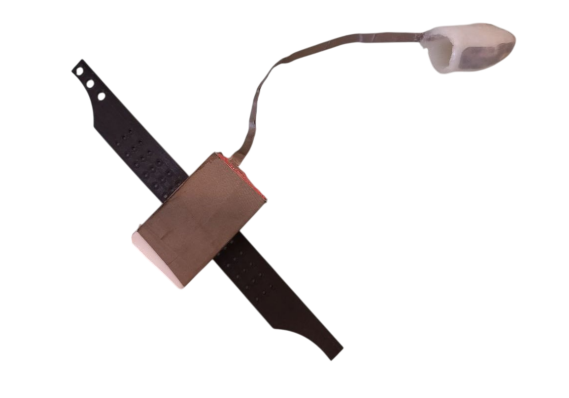
\includegraphics[width=0.6\textwidth]{SistemaDito.png}\\[0.3cm]
                    \caption{Sistema completo con pelle e interfaccia elettronica}
                    \label{fig:SistemaDito}
                \end{figure}

        \subsubsection{Matrice di sensori tattili}
            Lo sviluppo di sensori tattili basati su polimeri piezoelettrici è interessante per le loro proprietà fisiche
            e funzionali. Questi sensori offrono un'elevata sensibilità, sono sensori dinamici, in grado di misurare le
            variazioni delle pressioni applicate, e coprire un ampio intervallo di frequenze operative (da meno di 1 Hz
            fino a 1 kHz), coprendo l'intero spettro di frequenza dei meccanorecettori della pelle umana.
            Tra i materiali polimerici impiegati, il fluoruro di polivinilidene (PVDF) e i suoi copolimeri con trifluoroetilene (TrFE) si sono dimostrati particolarmente adatti per applicazioni tattili. 
            In particolare, il
            copolimero P(VDF-TrFE) presenta una combinazione di caratteristiche vantaggiose: elevata sensibilità
            piezoelettrica, che consente di rilevare anche pressioni minime; flessibilità meccanica, utile per l'integrazione su superfici curve o dispositivi indossabili; e stabilità piezoelettrica, 
            piroelettrica e ferroelettrica,
            che ne garantiscono l'affidabilità nel tempo. Tali proprietà lo rendono ideale per il rilevamento tattile
            dinamico e per l'integrazione in pelli elettroniche artificiali.\\

                \vspace{0.5cm}
                \begin{figure}[H]
                    \centering
                    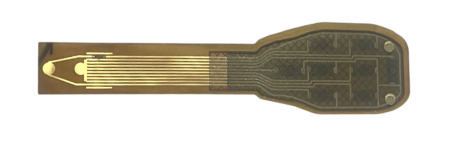
\includegraphics[width=0.5\textwidth]{MatriceSensori.png}\\[0.3cm]
                    \caption{Matrice di sensori}
                    \label{fig:MatriceSensori}
                \end{figure}

            La matrice di sensori, riportata in Figura~\ref{fig:MatriceSensori}, è realizzata tramite un processo di serigrafia, utilizzando
            il materiale P(VDF-TrFE) come strato attivo. Il processo produttivo prevede la deposizione serigrafica
            degli elettrodi inferiori su un substrato plastico trasparente e flessibile, in formato DIN A4. Successivamente, viene serigrafato uno strato di polimero ferroelettrico P(VDF-TrFE), 
            seguito dalla serigrafia degli
            elettrodi superiori. Un ulteriore strato di vernice indurente ai raggi UV viene applicato sulla superficie
            per proteggere il sensore da agenti esterni.
            Infine, viene eseguita una procedura di polarizzazione, necessaria per allineare lungo lo spessore i
            dipoli precedentemente orientati in modo casuale all'interno dei cristalliti del materiale. In Figura 3 è
            riportata la struttura di un singolo sensore\\

                \vspace{0.5cm}
                \begin{figure}[H]
                    \centering
                    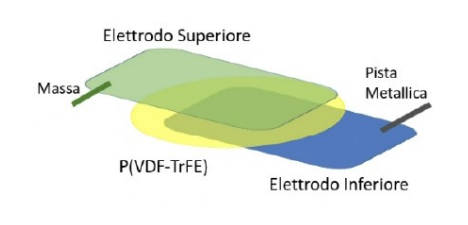
\includegraphics[width=0.5\textwidth]{SingoloSensore.png}\\[0.3cm]
                    \caption{ Struttura di un singolo sensore, uno strato di P(VDF-TrFE) posto tra due elettrodi}
                    \label{fig:StrutturaSensore}
                \end{figure}

            Il processo così descritto ha consentito la realizzazione di matrici sensoriali contenenti da 4 fino a 16
            sensori indipendenti. Il collegamento tra la pelle elettronica e l'interfaccia elettronica di lettura avviene
            mediante piste metalliche, successivamente protette da un nastro conduttivo. Infine, la matrice viene
            incapsulata nel silicone, al fine di renderla indossabile e di adattarla alla forma dell'indice di una mano.

        \subsubsection{Interfaccia elettronica}
            La Figura 4 mostra il circuito stampato (PCB) e il diagramma a blocchi relativi all'elettronica di interfaccia tra la matrice di sensori e il PC. Il circuito è composto da due 
            dispositivi commerciali principali: il
            modulo BL600 (Laird Connectivity, USA) per la connettività Bluetooth e il convertitore analogico-digitale
            a ingresso di corrente DDC232 (Texas Instruments, USA).

            Il PCB integra, sul lato inferiore, circuiti integrati digitali per la gestione dell'alimentazione (ad
            esempio, un regolatore di tensione) e un'interfaccia per il trasferimento dati via USB (es. FTDI232).
            L'architettura consente la gestione fino a 32 sensori tramite due connettori, ciascuno con 16 canali di
            ingresso. Entrambi i connettori sono collegati a un circuito di offset, anch'esso posizionato sul lato
            inferiore del PCB, il cui scopo è regolare la linea di base dei segnali bipolari generati dai sensori. In
            questo modo, il DDC232 è in grado di acquisire correttamente segnali sia a polarità positiva che negativa.
            Il chip DDC232 include più integratori corrente-tensione e convertitori analogico-digitali a modulazione delta-sigma. È configurato per operare con una risoluzione di 16 bit, in 
            modo da coprire l'intero
            intervallo di carica in ingresso. L'architettura del dispositivo consente il campionamento simultaneo dei
            32 canali di ingresso, con una frequenza configurabile fino a 6 kHz.\\
            Nel presente lavoro, l'elettronica è stata configurata per acquisire e trasmettere i dati di pressione provenienti
            da 8 sensori, a una frequenza di campionamento fissata a 2 kHz nel firmware dell'interfaccia.
            La pelle elettronica converte i contatti meccanici in segnali elettrici, generando un segnale per ciascun
            sensore. L'interfaccia elettronica campiona tali segnali e li converte in formato esadecimale, utilizzando 2
            byte per sensore, inoltre per ogni sensore viene calcolata la forza relativa ricostruita, anch'essa convertita in formato esadecimale con 2 byte per ogni sensore. 
            I dati relativi a tutti i sensori, acquisiti in un determinato istante temporale, vengono
            aggregati in un singolo pacchetto, rappresentato da una stringa di caratteri esadecimali.

            Ogni pacchetto inizia con un'intestazione fissa, denominata Header di 3 byte e pari a 0x3C3E00, seguita dal numero di canali utilizzati, rappresentato da 1 byte, il timestamp 
            che identifica l'istante temporale associato a ciascun campione e permette di ricostruire l'andamento del segnale nel tempo,
            espresso in microsecondi, rappresentato da 4 byte e dai dati acquisiti dei sensori che sono rappresentati da 16 byte nel caso di 8 canali, uno per ciascun sensore.
            Il singolo pacchetto trasmesso 
            tramite protocollo seriale al PC ha 
            un peso complessivo di 24 byte nella configurazione utilizzata per la sola trasmissione dei dati grezzi. 
            La struttura del pacchetto è stata successivamente adattata nel corso dello sviluppo del sistema per includere anche i valori di forza relativa ricostruita dal sistema embedded, aggiungendo
            ulteriori 16 byte portando il pacchetto al peso complessivo di 40 byte.

        \subsection{Algoritmo per la ricostruzione della forza relativa}
            In questa sezione viene analizzato nei dettagli l'algoritmo per la ricostruzione della forza relativa

            \subsubsection{Principio di funzionamento}
                L'algoritmo di ricostruzione ha lo scopo di ottenere una stima della forza relativa applicata ai singoli sensori a partire dai segnali elettrici acquisiti. Poiché 
                la risposta dei sensori piezoelettrici è intrinsecamente dinamica e proporzionale alla derivata della pressione applicata, il segnale 
                grezzo non fornisce direttamente il valore della forza statica esercitata. È pertanto necessaria un'elaborazione digitale in grado di identificare
                gli eventi di contatto e di integrarne il contributo nel tempo per ricavarne un'indicazione quantitativa.
                
                L'elaborazione viene 
                effettuata considerando sia il comportamento dei singoli sensori sia quello complessivo della matrice. Per ciascun sensore, l'algoritmo analizza il segnale acquisito e 
                determina inizialmente una condizione di riferimento in assenza di pressione. A partire da tale condizione vengono definite delle soglie utilizzate per distinguere le variazioni 
                dovute a una pressione effettivamente applicata dalle normali oscillazioni del segnale. Parallelamente, i segnali dei diversi sensori vengono considerati attraverso una logica globale, 
                utilizzata per caratterizzare l'attività complessiva della matrice e supportare il rilevamento degli eventi di pressione. 
                Quando vengono rilevate le condizioni associate a un 
                evento di pressione, l'algoritmo ne analizza l'andamento nel tempo mediante l'integrazione, o accumulo, del segnale oppurtunamente filtrato.
                Il valore ottenuto viene successivamente normalizzato rispetto al massimo valore accumulato raggiunto durante l'evento, ottenendo una forza relativa compresa nell'intervallo
                $[0,1]$. Il rilevamento e la 
                gestione dell'evento sono inoltre regolati mediante una macchina a stati finiti, che consente di distinguere le diverse fasi della pressione, corrispondenti alle condizioni di assenza di 
                pressione, inizio della pressione, mantenimento e rilascio.
                L'intero procedimento viene eseguito in tempo reale per ciascuno degli otto sensori, utilizzando anche le informazioni
                globali ricavate dalla matrice, e consente di ottenere un vettore di forze relative istantanee per ogni canale.

            \subsubsection{Calibrazione e determinazione della condizione di fondo}
                L'algoritmo utilizza un insieme di parametri configurabili che consentono di adattarne il funzionamento alle caratteristiche dei segnali acquisiti e alle condizioni operative
                del sistema. Il numero di sensori \texttt{N\_Sensors}, è personalizzabile in funzione dell'interfaccia utilizzata, mentre gli altri parametri regolano le modalità
                di calibrazione, filtraggio, rilevamento e ricostruzione del segnale.

                Una prima fase dell'elaborazione è dedicata alla determinazione delle condizioni di fondo del sistema, necessaria per distinguere le variazioni del segnale associate a una pressione 
                effettiva dalle oscillazioni dovute al rumore e alla deriva dei sensori.
                Durante la fase iniziale di avvio vengono acquisiti alcuni campioni in assenza di pressione, utilizzati per caratterizzare il comportamento del segnale.
                
                Il parametro \texttt{Warmup\_Samples} definisce il numero di campioni iniziali che vengono esclusi dall'elaborazione. Questa fase di warm-up permette di evitare che eventuali 
                transitori presenti immediatamente dopo l'avvio vengano interpretati come variazioni significative del segnale. Successivamente, il parametro \texttt{Threshold\_Samples} stabilisce il numero 
                di campioni utilizzati per la fase di apprendimento del rumore di fondo. I campioni acquisiti durante questa fase vengono impiegati per determinare, per ciascun sensore, 
                i valori necessari alla definizione della soglia di rilevamento e dell'offset.
                
                Il parametro \texttt{Alpha} determina il comportamento del filtro passa-basso esponenziale applicato al segnale. Il filtro realizza una 
                media pesata tra il campione corrente e l'informazione precedente, attenuando variazioni rapide e contribuendo a ridurre l'influenza di spike, vibrazioni meccaniche e disturbi
                elettronici. Il carattere esponenziale del filtro deriva dalla progressiva riduzione del peso attribuito ai campioni più lontani nel tempo.
                Questo filtro è caratterizzato dalla seguente equazione:

                    \begin{equation}
                        y(n) = \alpha x_{raw}(n) + (1 - \alpha) \cdot y(n-1)
                    \end{equation}
                
                Dove $x_{raw}(n)$ indica il segnale grezzo acquisito dal sensore, $\alpha$ indica proprio il parametro \texttt{Alpha} e l'uscita $y(n)$ del filtro costituisce il segnale utilizzato nelle successive fasi di elaborazione. 
                Prima del rilevamento degli eventi di pressione, tale segnale viene corretto
                per compensare la componente continua dovuta all'offset dei sensori.
                Per la stima della componente continua del segnale vengono considerati gli ultimi
                \texttt{nSamples\_Adaptive\_Offset} (numero di campioni per l'offset adattivo), campioni della fase di apprendimento. A partire da essi viene calcolato il valore medio, utilizzato come \texttt{Adaptive Offset}. 
                Il segnale viene quindi corretto sottraendo tale valore: 

                    \begin{equation}
                        x_{\mathrm{corretto}}(n) =
                        y(n) -
                        \mathrm{Adaptive\_Offset}
                    \end{equation}

                Per caratterizzare il rumore presente sui diversi canali, viene inizialmente calcolata, per ciascun sensore, la mediana dei campioni acquisiti durante la fase di apprendimento. 
                La mediana viene utilizzata come valore centrale del segnale di rumore, risultando meno sensibile rispetto alla media alla presenza di eventuali valori anomali. 
                A partire dagli stessi campioni viene inoltre calcolata la deviazione standard campionaria $\sigma$, che rappresenta la variabilità del rumore rispetto al valore centrale.
                
                Per determinare la soglia oltre la quale il segnale viene considerato indicativo di una pressione, l'algoritmo utilizza il parametro configurabile \texttt{Press Sigma}. 
                Tale parametro rappresenta il numero di deviazioni standard utilizzato per separare il rumore di fondo da una variazione significativa del segnale. La soglia di pressione viene 
                quindi calcolata individualmente per ciascun sensore secondo:

                    \begin{equation}
                        \mathrm{Soglia} =
                        \mathrm{Press\_Sigma} \cdot \sigma
                    \end{equation}

                Il parametro \texttt{Press\_Sigma} consente quindi di regolare la sensibilità del rilevamento: valori più elevati rendono necessaria una variazione maggiore del segnale per attivare il 
                rilevamento di una pressione, mentre valori più bassi rendono il sistema più sensibile alle variazioni del segnale. Poiché la deviazione standard viene calcolata separatamente per 
                ciascun sensore, la soglia si adatta inoltre alle caratteristiche di rumore dei singoli canali.

                La separazione tra la stima del valore centrale del rumore e quella dell'offset consente quindi di caratterizzare separatamente la componente variabile del segnale, 
                descritta dalla deviazione standard, e la sua componente continua, rappresentata dall'offset.

                Il parametro \texttt{Press\_Confirm} definisce il numero di campioni consecutivi che devono soddisfare la condizione di superamento della soglia affinché un evento venga
                considerato una pressione effettiva. Questa condizione permette di evitare che variazioni isolate del segnale o spike di breve durata vengano interpretati come eventi di pressione.

                Durante la fase di pressione, il parametro \texttt{NW} definisce la durata della finestra di elaborazione, espressa in numero di campioni. Per ogni campione appartenente a 
                tale intervallo, l'algoritmo esegue l'integrazione discreta del modulo del segnale corretto:

                    \begin{equation}
                        I(n) = I(n-1) + |x_{\mathrm{corretto}}(n)|
                    \end{equation}

                L'accumulatore $I(n)$ rappresenta quindi la grandezza energetica legata all'andamento e all'intensità del segnale durante l'evento di pressione e viene successivamente utilizzato per 
                la ricostruzione della forza relativa. Al termine della finestra \texttt{NW}, l'algoritmo verifica inoltre la presenza di una condizione di pressione globale, 
                distinguendo un evento potenzialmente dovuto al rumore da una pressione valida.

                La gestione degli eventi tiene inoltre conto del comportamento complessivo della matrice attraverso uno stato globale del sistema. Oltre allo stato locale associato a ciascun sensore, 
                l'algoritmo considera il numero di sensori che rilevano contemporaneamente una condizione di pressione. Il parametro \texttt{Min\_Press\_Sensors} stabilisce il numero minimo di 
                sensori attivi necessario per validare globalmente un evento. Questa logica consente di ridurre i falsi positivi dovuti all'attivazione accidentale di un singolo sensore, assumendo
                che una pressione reale esercitata sulla pelle artificiale coinvolga generalmente più elementi della matrice.

                Una volta attivata la condizione globale, l'algoritmo impedisce temporaneamente l'attivazione di nuovi eventi locali, evitando che ulteriori variazioni dei sensori vengano
                interpretate come eventi indipendenti durante la stessa pressione.

                Durante la fase di rilascio, l'integrale accumulato viene progressivamente ridotto in funzione del segnale rilevato. Un sensore viene considerato rilasciato quando il proprio integrale 
                scende al di sotto del 50\% del massimo valore raggiunto durante l'evento. Il parametro \texttt{Release\_Ratio} definisce invece la frazione dei sensori coinvolti nella pressione 
                globale che deve essere riconosciuta come rilasciata affinché l'evento globale venga terminato e il sistema venga riportato alla condizione iniziale.

                Il parametro \texttt{Sample\_After\_Release} introduce infine un intervallo di guardia, espresso in campioni, successivo al 
                rilascio, durante il quale il sensore non viene considerato per il rilevamento di un nuovo evento, riducendo la possibilità che oscillazioni residue del segnale vengano
                interpretate come una nuova pressione.

            \subsubsection{Rilevamento dell'evento di pressione}
                Una volta completata la fase di calibrazione, l'algoritmo utilizza il segnale corretto $x_{\mathrm{corretto}}(n)$ per individuare l'eventuale presenza di un evento di pressione. 
                Il rilevamento viene eseguito in modo indipendente per ciascun sensore, confrontando il valore assoluto del segnale filtrato con la soglia di attivazione precedentemente determinata:

                    \begin{equation}
                    |x_{\mathrm{corretto}}(n)| > \mathrm{Soglia}
                    \end{equation}

                Il superamento della soglia da parte di un singolo campione non è tuttavia sufficiente per considerare l'evento come una pressione effettiva. Per evitare che variazioni isolate 
                del segnale vengano interpretate come eventi validi, viene utilizzato il parametro \texttt{Press\_Confirm}, che richiede il superamento della soglia per un numero consecutivo di campioni. 
                Quando tale condizione viene soddisfatta, il sensore viene considerato localmente in fase di pressione.

                La gestione dell'evento è realizzata mediante una macchina a stati finiti (Finite State Machine, FSM) il cui funzionamento viene approfondito nella seguente sottosezione.

                La condizione di pressione non viene valutata esclusivamente a livello del singolo sensore, ma anche considerando il comportamento complessivo della matrice. A tale scopo, 
                l'algoritmo considera uno stato globale che tiene conto del numero di sensori che hanno rilevato contemporaneamente un evento di pressione. Il parametro \texttt{Min\_Press\_Sensors} 
                stabilisce il numero minimo di sensori che devono risultare attivi affinché venga riconosciuta una condizione di pressione globale.

                Quando tale condizione viene raggiunta, l'evento viene considerato valido a livello della matrice e per i sensori coinvolti si prosegue nell'elaborazione dell'evento. 
                Durante questa fase, l'attivazione di nuovi eventi locali viene temporaneamente impedita, in modo da evitare che variazioni successive degli altri sensori vengano interpretate 
                come eventi distinti appartenenti alla stessa pressione.

                La combinazione tra il rilevamento locale e la validazione globale permette quindi di distinguere le variazioni isolate, potenzialmente dovute al rumore, dagli eventi che 
                coinvolgono un numero significativo di sensori della pelle artificiale. La macchina a stati consente inoltre di seguire l'intero ciclo dell'evento, dalla sua attivazione fino al rilascio, 
                fornendo le condizioni necessarie per la successiva ricostruzione della forza relativa.

            \subsubsection{Macchina a stati finiti}
                La gestione temporale degli eventi di pressione è realizzata mediante una macchina a stati finiti (Finite State Machine, FSM), che permette di rappresentare in modo strutturato 
                le diverse fasi attraversate da ciascun sensore durante un evento. Ogni sensore dispone di uno stato locale, aggiornato in funzione dell'andamento del segnale e delle condizioni di 
                rilevamento precedentemente descritte. Gli stati considerati sono \texttt{IDLE}, \texttt{PRESS}, \texttt{HOLD} e \texttt{RELEASE}.
                    
                    \begin{itemize}

                        \item \textbf{\texttt{IDLE}:} Stato di riposo in assenza di pressione. In questa fase il sensore viene monitorato continuamente e, quando il segnale supera la soglia 
                        per un numero di campioni consecutivi pari a \texttt{Press\_Confirm}, viene avviata una nuova fase di pressione e il sensore passa allo stato \texttt{PRESS}.

                        \item \textbf{\texttt{PRESS}:} Fase di innesco e analisi iniziale dell'evento. Il segnale corretto viene accumulato secondo la modalità descritta nel sottocapitolo precedente 
                        e viene verificata la presenza di una condizione di pressione globale. Al termine della finestra temporale definita da \texttt{NW}, l'algoritmo determina se l'attività rilevata 
                        può essere associata a un evento di pressione valido. Se non è presente una condizione globale, l'evento viene considerato potenzialmente dovuto al rumore e il sensore viene riportato 
                        allo stato \texttt{IDLE}. In caso contrario, il sensore passa allo stato \texttt{HOLD}.

                        \item \textbf{\texttt{HOLD}:} Fase di regime. In questa fase l'accumulatore continua l'integrazione del segnale e salva il 
                        valore massimo raggiunto durante l'evento (indicato come $I_{\mathrm{max}}$), il quale viene mantenuto come riferimento per la successiva normalizzazione della forza relativa. Il sensore rimane nello stato \texttt{HOLD} fino a 
                        quando le condizioni associate al rilascio non vengono soddisfatte.

                        \item \textbf{\texttt{ RELEASE}:} Fase di rilascio del contatto. Quando il segnale associato all'evento diminuisce, l'accumulatore viene progressivamente ridotto in funzione 
                        del valore del segnale rilevato. Il rilascio del singolo sensore viene considerato completato quando l'integrale accumulato scende al di sotto del 50\% del massimo valore 
                        raggiunto durante l'evento. Il sensore viene quindi riportato alla condizione \texttt{IDLE}, tenendo conto dell'intervallo di guardia definito dal parametro \texttt{Sample\_After\_Release}.

                    \end{itemize}


                Oltre agli stati locali, l'algoritmo supervisiona uno stato globale della matrice, utilizzato per determinare se l'attività rilevata dai singoli sensori corrisponde a un unico evento 
                di pressione. La condizione globale viene attivata quando il numero di sensori che hanno rilevato una pressione raggiunge almeno il valore definito da \texttt{Min\_Press\_Sensors}. 
                Una volta attivata, la condizione globale impedisce temporaneamente l'attivazione di nuovi eventi locali, così da considerare le successive variazioni dei sensori come parte dello
                stesso evento.

                Durante il rilascio, lo stato globale viene mantenuto fino a quando una frazione sufficiente dei sensori coinvolti nell'evento viene riconosciuta come rilasciata. 
                Tale frazione è determinata dal parametro \texttt{Release\_Ratio}. Quando la condizione viene soddisfatta, l'evento globale viene terminato e il sistema può tornare 
                alla condizione iniziale, consentendo il rilevamento di un nuovo evento.

                La combinazione tra stati locali e stato globale permette quindi di gestire l'intero ciclo di pressione, tenendo conto sia dell'evoluzione temporale del segnale di ciascun 
                sensore sia dell'attività complessiva della matrice.

            \subsubsection{Ricostruzione della forza relativa}

                Una volta riconosciuto e validato un evento di pressione, l'algoritmo utilizza l'integrale discreto associato a ciascun sensore per ottenere una misura relativa dell'intensità dell'evento. 
                Come descritto nei sottocapitoli precedenti, durante le fasi di pressione e mantenimento viene accumulato il valore assoluto del segnale corretto, ottenendo una grandezza $I(n)$ che
                descrive l'andamento del segnale durante l'evento.

                Per ciascun sensore viene inoltre mantenuto il massimo valore raggiunto dall'accumulatore durante l'evento, indicato come $I_{\mathrm{max}}$. Tale valore costituisce il riferimento 
                utilizzato per la normalizzazione del segnale. La forza relativa viene quindi calcolata secondo:

                    \begin{equation}
                    F_{\mathrm{rel}}(n) =
                    \frac{I(n)}{I_{\mathrm{max}}}
                    \end{equation}

                Il valore ottenuto è compreso nell'intervallo $[0,1]$, dove valori prossimi a zero corrispondono a una bassa intensità del segnale associato all'evento, mentre valori prossimi a 
                uno corrispondono al massimo livello raggiunto dal sensore durante l'evento considerato. La normalizzazione consente quindi di esprimere il livello di attivazione del singolo sensore 
                in forma relativa, indipendentemente dal valore assoluto dell'accumulatore.

                La ricostruzione viene effettuata separatamente per ciascun canale della matrice, permettendo di ottenere contemporaneamente otto valori di forza relativa, uno per ciascun sensore 
                utilizzato nel sistema. Durante la fase di rilascio, l'accumulatore viene progressivamente ridotto e, di conseguenza, anche il valore di forza relativa diminuisce fino alla conclusione
                dell'evento.

                Il valore di forza relativa ottenuto costituisce infine l'uscita dell'algoritmo di ricostruzione e può essere trasmesso in tempo reale al sistema di elaborazione esterno insieme ai 
                dati acquisiti dai sensori.

        \subsection{Iter di sviluppo del sistema}
            La ricostruzione della forza relativa a partire dai segnali provenienti dai sensori piezoelettrici e la sua successiva elaborazione in tempo reale su microcontrollore hanno
            richiesto diverse fasi di sviluppo. Inizialmente, l'algoritmo per la ricostruzione della forza relativa è stato sviluppato in Python sotto forma di classe, per essere successivamente 
            adattato e implementato in linguaggio C per microcontrollore.
            L'iter di sviluppo può essere suddiviso nelle seguenti fasi:

            \begin{enumerate}
                \item Acquisizione dei segnali provenienti dai sensori tramite il software LabVIEW e realizzazione di un programma Python per il plotting degli stessi;
                \item Verifica del funzionamento dell'algoritmo di ricostruzione della forza relativa, in modalità offline, sui segnali precedentemente acquisiti, mediante lo sviluppo di un programma Python;
                \item Sviluppo di un programma Python per l'acquisizione in tempo reale dei dati grezzi provenienti dai sensori e la successiva visualizzazione offline;
                \item Porting e implementazione dell'algoritmo di ricostruzione della forza relativa sul microcontrollore integrando il firmware esistente;
                \item Acquisizione in tempo reale dei dati grezzi e dei valori di forza relativa ricostruiti dal microcontrollore, mediante la modifica del precedente script Python.
            \end{enumerate}
            
            Le diverse fasi hanno permesso di procedere progressivamente dall'analisi preliminare dei segnali all'integrazione 
            dell'intero processo di acquisizione ed elaborazione sul sistema embedded. Nelle sottosezioni successive vengono descritte le singole fasi di sviluppo e le relative modalità di implementazione.

            \subsubsection{Acquisizione e visualizzazione dei dati}
                In questa prima fase di sviluppo del sistema, l'acquisizione dei dati provenienti dai sensori piezoelettrici è stata effettuata mediante il software \textit{LabVIEW}, utilizzato per l'interfacciamento
                con il sistema di acquisizione e registrazione dei segnali.

                L'obiettivo di questa fase consisteva nell'analizzare il comportamento dei sensori, osservare l'andamento temporale dei segnali acquisiti e individuare le variazioni 
                associate all'applicazione di una pressione. Le acquisizioni sono state effettuate utilizzando una frequenza di 
                campionamento  $f_s = 2\,\mathrm{kHz}$, registrando 4000 campioni per ciascun canale, corrispondenti a una durata complessiva di 2 secondi.

                I dati acquisiti tramite \textit{LabVIEW} sono stati salvati in file in formato \texttt{.csv}, organizzati con una struttura a 4000 righe, corrispondenti ai campioni
                acquisiti e 9 colonne: la prima colonna riporta il \textit{timestamp} associato a ciascun campione, mentre le restanti otto 
                contengono i dati provenienti dagli 8 canali dei sensori piezoelettrici. Tale struttura dati è stata mantenuta anche per le successive fasi di sviluppo.

                Per la visualizzazione dei dati è stato sviluppato un programma in Python in grado di importare i file \texttt{.csv} e rappresentare graficamente 
                l'andamento temporale dei segnali relativi agli otto sensori. La visualizzazione simultanea dei diversi canali ha permesso di confrontare 
                le risposte dei sensori e di osservare le variazioni dei segnali durante gli eventi di pressione.

                Un aspetto rilevante di questa prima configurazione è che i dati registrati nei file \texttt{.csv} relativi ai segnali risultano già convertiti in volt,
                quindi il programma di visualizzazione ha potuto utilizzare direttamente i valori acquisiti senza necessità di conversione dal valore in uscita dal
                convertitore analogico-digitale (DDC232).

                Questa prima fase ha costituito il punto di partenza per le successive attività di sviluppo, fornendo i dati necessari per caratterizzare 
                preliminarmente il comportamento dei sensori e procedere alla 
                successiva implementazione e verifica dell'algoritmo di ricostruzione della forza.\\

                %immagine labview + immagine segnali raw
                

            \subsubsection{Ricostruzione della forza relativa offline}
                Una volta ottenute e verificate graficamente le prime acquisizioni dei segnali, si è proceduto alla prima implementazione del ricostruttore 
                della forza relativa in ambiente Python. L'obiettivo di questa fase era verificare il comportamento dell'algoritmo offline, utilizzando i dati 
                reali acquisiti precedentemente.

                La classe \texttt{ForceReconstructor} è stata integrata nello script di visualizzazione grafica, consentendo di sovrapporre sullo stesso grafico i
                segnali acquisiti e la rispettiva forza relativa normalizzata. Questo approccio è risultato essenziale per la taratura e l'ottimizzazione dei 
                parametri del ricostruttore.

                La versione offline ha stabilito il comportamento di riferimento per le successive fasi di sviluppo. Poiché i dati elaborati 
                rispecchiavano fedelmente il formato di quelli poi trasmessi in tempo reale dal sistema embedded, questa fase ha garantito una solida base 
                di confronto per la successiva implementazione in linguaggio C.

                La verifica offline del ricostruttore ha costituito quindi il primo risultato completo del sistema e ha definito il comportamento di riferimento per le 
                successive fasi di sviluppo. Questa implementazione ha fornito una cartina tornasole per il confronto 
                con i risultati ottenuti durante l'elaborazione in tempo reale. 

                %immagine segnali raw da labview + forza ricostruita
                \vspace{0.5cm}
                \begin{figure}[H]
                    \centering
                    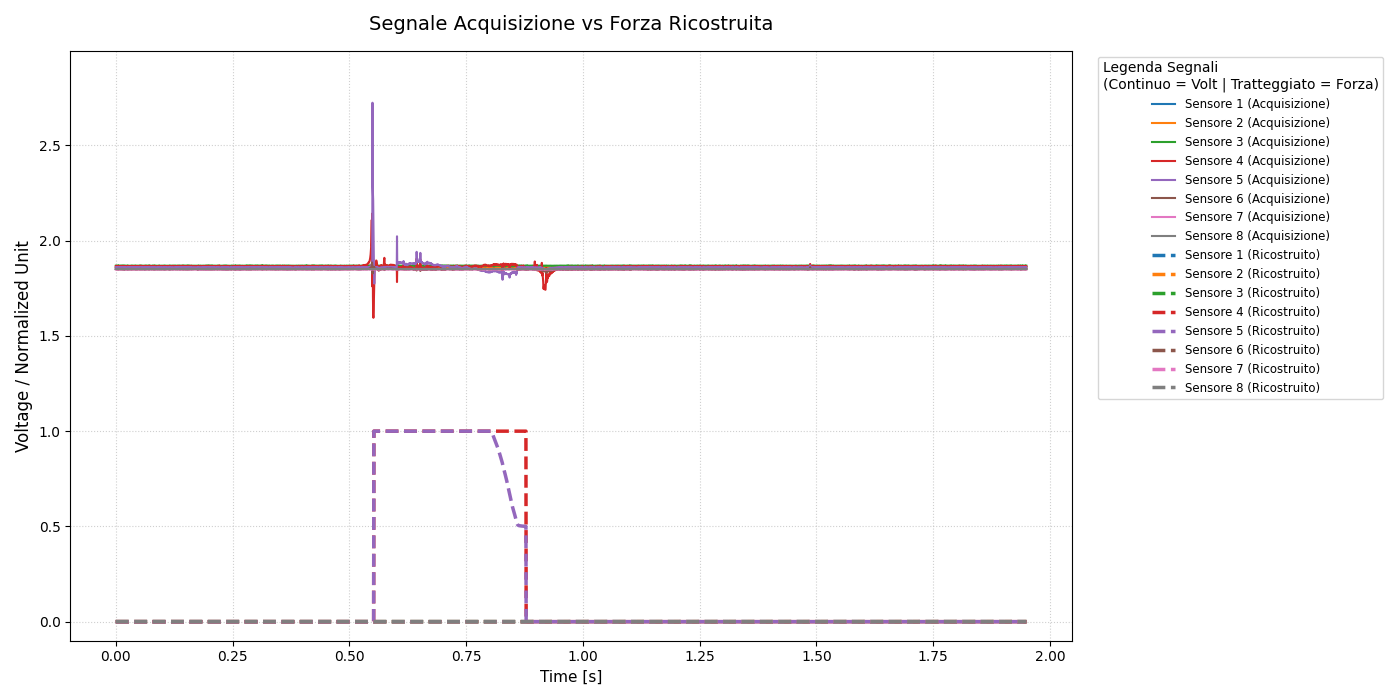
\includegraphics[width=1\textwidth]{LabviewRicostruttore.png}\\[0.3cm]
                    \caption{Prova del ricostruttore offline sui segnali acquisiti da LabVIEW}
                    \label{fig:LabRic}
                \end{figure}

                In Figura~\ref{fig:LabRic} viene illustrato il primo risultato dell'intero processo di sviluppo: la linea continua mostra il segnale proveniente
                dai sensori mentre quella tratteggiata la forza relativa ricostruita. Si nota come l'andamento della forza relativa ricostruita segue quello del segnale:
                al picco che indica la pressione corrisponde la salita ripida del segnale del ricostruttore che rimane al suo valore di plateu (1) fino al rilevamento del
                secondo picco del segnale, che indica il rilascio e quindi la fine della pressione.

            \subsubsection{Acquisizione dei dati in tempo reale}
                L'obiettivo di questa fase era realizzare l'acquisizione in tempo reale dei dati provenienti dai sensori direttamente sul PC tramite comunicazione 
                seriale,
                eliminando il passaggio intermedio costituito da \textit{LabVIEW}. 

                In questa ottica è stato sviluppato un programma in Python dedicato alla gestione della comunicazione con il microcontrollore e alla ricezione e 
                salvataggio dei dati acquisiti.

                La comunicazione tra il microcontrollore e il PC è stata configurata mediante interfaccia UART con una velocità di trasmissione pari a $3\,\mathrm{Mbps}$. 
                Il programma Python gestisce l'intero ciclo di acquisizione, dalla richiesta di avvio fino alla ricezione e al salvataggio dei dati relativi ai 
                4000 campioni.

                L'acquisizione viene avviata mediante l'invio al microcontrollore di un comando di \texttt{start}, seguito dall'indicazione dei canali da utilizzare, secondo il 
                formato \texttt{start,1-8}. Il comando permette al firmware di avviare la comunicazione e di configurare il numero di sensori coinvolti nell'acquisizione.

                Una volta avviata la comunicazione, il programma Python ricerca e interpreta i pacchetti ricevuti dalla porta seriale. Per ogni pacchetto 
                vengono identificati l'header, 
                il numero di canali e il timestamp, seguiti dai campioni provenienti dai convertitori ADC. I dati dei canali vengono quindi estratti dal flusso
                di byte e convertiti nel corrispondente formato numerico mediante la funzione \texttt{unpack()}. In particolare, viene utilizzato il formato 
                \texttt{big-endian} per interpretare correttamente l'ordine dei byte con cui i campioni sono presenti nel pacchetto ricevuto.
                La necessità di specificare l'ordine dei byte deriva dal formato con cui i dati digitali vengono forniti dall'interfaccia del convertitore. 
                I byte che costituiscono ciascun campione devono infatti essere ricomposti nell'ordine corretto prima di poter ottenere il valore numerico 
                del campione. Il programma Python esegue quindi la conversione dal flusso di byte ricevuto al valore intero associato a ciascun canale, rendendo 
                i dati disponibili per le successive elaborazioni.

                I dati ricevuti vengono salvati su file \texttt{.csv} separati, mantenendo sia i valori nel formato RAW acquisito, 
                sia i corrispondenti valori convertiti in volt. 
                Per la conversione dei valori ADC in volt viene utilizzata la seguente formula: 

                    \begin{equation}
                        V_{\mathrm{ch}} = \frac{C_{\mathrm{ADC}} \cdot V_{\mathrm{REF}}}{\mathrm{ADC}_{\mathrm{MAX}}}
                    \end{equation}
                
                Dove $V_{\mathrm{ch}}$ rappresenta il valore di tensione corrispondente al campione del canale, $C_{\mathrm{ADC}}$ rappresenta il codice digitale del campione 
                ADC, ovvero il valore RAW ricevuto, $\mathrm{ADC}_{\mathrm{MAX}}$ rappresenta il valore massimo del codice digitale considerato, pari a 65535 
                nel formato \texttt{uint16\_t}, mentre $V_{\mathrm{REF}}$ indica la tensione di riferimento dell'ADC, pari a $4.096\,\mathrm{V}$.

                Al termine dell'acquisizione viene inviato il comando di arresto della comunicazione seriale. I dati così ottenuti vengono quindi forniti 
                al programma per la ricostruzione della forza relativa offline sviluppato nella fase precedente.
                In questo modo è possibile applicare l'algoritmo già verificato sui dati acquisiti in precedenza, ma utilizzando questa volta 
                segnali ottenuti direttamente in tempo reale dal sistema.

                Questa configurazione ha permesso di verificare il comportamento della catena di acquisizione in condizioni operative reali, valutando 
                la corretta ricezione dei pacchetti, la corrispondenza tra i canali dei sensori e la corretta successione temporale dei campioni. La possibilità 
                di applicare il ricostruttore già verificato ai dati acquisiti condizioni operative reali e ha inoltre permesso di verificare che il nuovo sistema di 
                acquisizione producesse dati compatibili con quelli visti nella precedente fase.

                Il completamento di questa fase ha costituito il punto di partenza per il successivo porting dell'algoritmo dal linguaggio Python al linguaggio 
                C e per la sua integrazione direttamente nel firmware del microcontrollore.

            \subsubsection{Porting dell'algoritmo sul microcontrollore}
                In questa fase di sviluppo del sistema si è proceduto al porting dell'algoritmo
                dall'ambiente Python al linguaggio C, con l'obiettivo di eseguire direttamente sul microcontrollore la ricostruzione della forza relativa.

                L'implementazione in C è stata sviluppata mantenendo invariata la logica di elaborazione definita nella precedente implementazione Python. Sono 
                state quindi riprodotte le principali operazioni dell'algoritmo, comprendenti la calibrazione dei sensori, il filtraggio dei segnali, 
                il calcolo delle soglie, il rilevamento degli eventi di pressione, l'aggiornamento delle grandezze interne e la gestione della macchina a stati finiti. 
                La descrizione dettagliata di tali operazioni è riportata nella sezione dedicata al funzionamento dell'algoritmo.

                Il passaggio al linguaggio C ha richiesto l'adattamento dell'algoritmo alla struttura del firmware e alle modalità di elaborazione proprie del microcontrollore. 
                In particolare, l'elaborazione è stata organizzata in modo sequenziale, così che a ogni nuovo campione acquisito vengano aggiornati i dati e lo 
                stato interno degli otto sensori. Il ricostruttore opera quindi direttamente sui campioni ricevuti tramite l'interfaccia SPI, senza richiedere 
                l'elaborazione preliminare dei dati da parte del PC.

                Prima dell'integrazione definitiva nel firmware, la corretta corrispondenza tra le due implementazioni è stata verificata mediante un apposito 
                \textit{wrapper} Python. L'implementazione C del ricostruttore è stata richiamata dall'ambiente Python e sottoposta agli stessi dati utilizzati 
                precedentemente per la verifica offline dell'algoritmo. I risultati ottenuti dall'implementazione in C sono stati quindi confrontati con quelli 
                prodotti dalla classe \texttt{ForceReconstructor} sviluppata in Python. Questa procedura ha permesso di verificare che il porting mantenesse il 
                comportamento dell'algoritmo originale prima del suo utilizzo durante l'acquisizione sul microcontrollore. Per vedere nel dettaglio le differenze
                tra le due implementazioni si veda Figura~\ref{fig:confronto_immagini}.

                %immagini del terminal e grafico sulle discrepanze tra ricostruttore C e Python
                \begin{figure}[H]
                    \centering
                    % Prima immagine (occupa il 48% della larghezza del testo)
                    \begin{subfigure}[b]{0.35\textwidth}
                        \centering
                        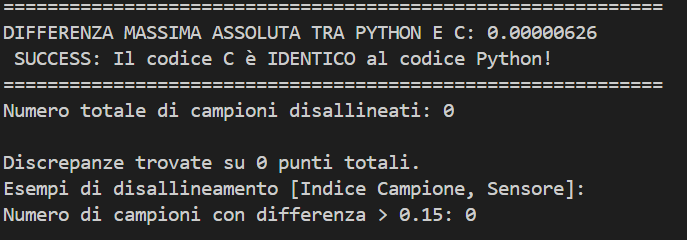
\includegraphics[width=\textwidth]{Discrepanze.png}
                        \caption{Percentuali e valori indicativi delle discrepanze nel confronto tra i due ricostruttori.}
                        \label{fig:terminal}
                    \end{subfigure}
                    \hfill % Spazio orizzontale flessibile per separare le due immagini
                    % Seconda immagine (occupa il 48% della larghezza del testo)
                    \begin{subfigure}[b]{0.61\textwidth}
                        \centering
                        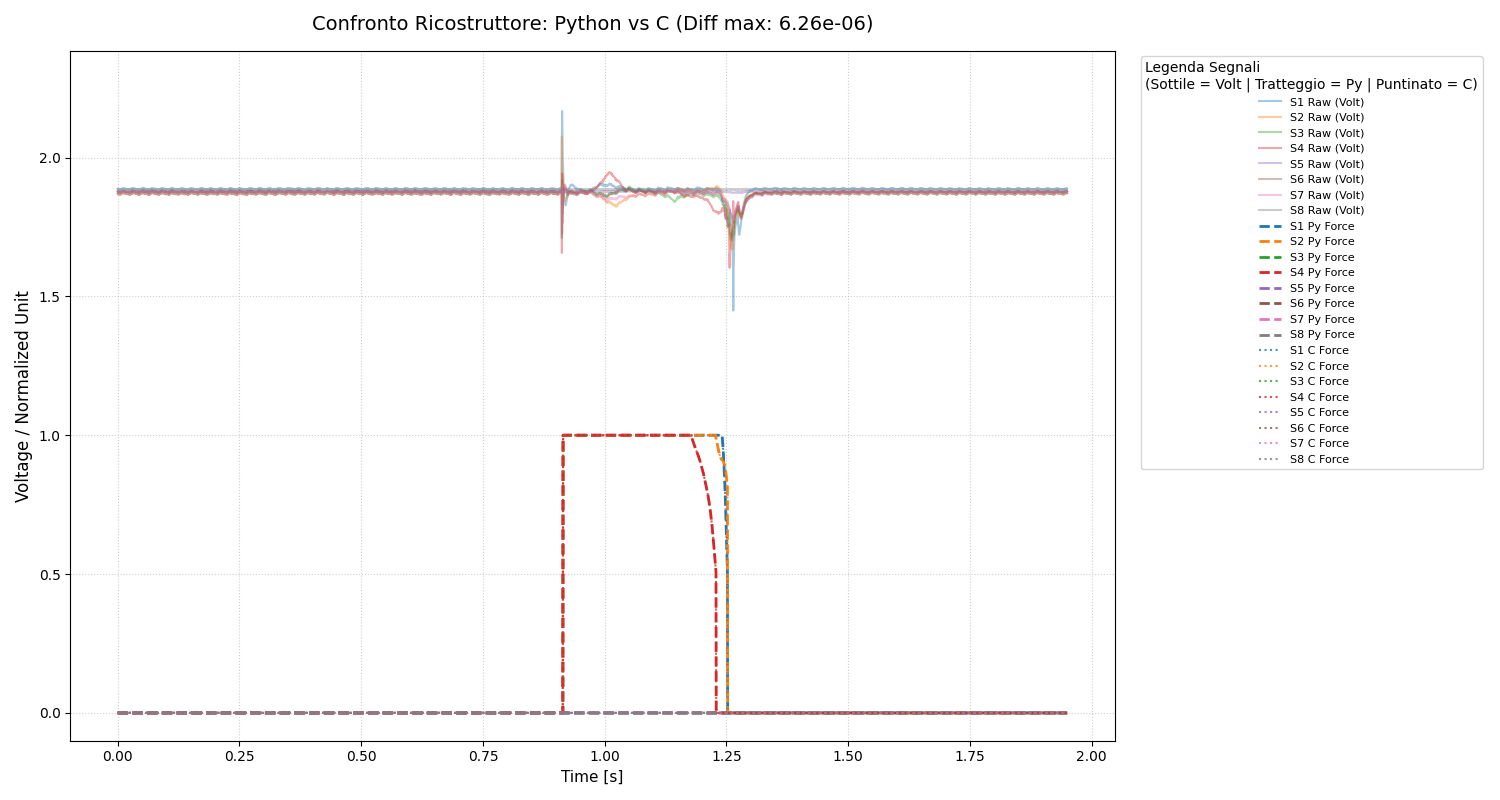
\includegraphics[width=\textwidth]{DiscrepanzeCpy.png}
                        \caption{Confronto grafico e sovrapposizione delle risposte}
                        \label{fig:seconda_immagine}
                    \end{subfigure}
                    % Didascalia generale e label della figura complessiva
                    \caption{Confronto tra ricostruttore Python e ricostruttore C}
                    \label{fig:confronto_immagini}
                \end{figure}

                Una volta verificata la corrispondenza tra le due implementazioni, il ricostruttore in C è stato integrato nel firmware dello STM32H742. I 
                campioni acquisiti vengono elaborati direttamente a bordo del microcontrollore e, per ciascun sensore, vengono aggiornate le grandezze interne 
                dell'algoritmo e il relativo stato dell'evento di pressione. Il valore di forza relativa prodotto dal ricostruttore viene quindi reso disponibile
                per la successiva trasmissione al PC insieme ai dati acquisiti.

                L'integrazione del ricostruttore nel firmware ha permesso di spostare l'elaborazione dal PC al microcontrollore, completando il passaggio da una 
                ricostruzione eseguita offline o sul computer a una ricostruzione effettuata direttamente durante l'acquisizione dei dati.
                
                

            \subsubsection{Modifiche e integrazione del firmware}
                L'integrazione dell'algoritmo di ricostruzione all'interno del firmware ha richiesto alcune modifiche alla gestione dei dati acquisiti e al 
                flusso di elaborazione, con l'obiettivo di eseguire la ricostruzione direttamente sul microcontrollore e predisporre i dati per la successiva 
                trasmissione al PC.

                L'elaborazione dei campioni acquisiti viene eseguita all'interno della funzione \texttt{HAL\_SPI\_RxCpltCallback}, richiamata al completamento 
                della ricezione tramite interfaccia SPI. Per evitare che i dati presenti nel buffer di ricezione possano essere sovrascritti durante la loro 
                elaborazione, viene innanzitutto realizzata una copia dei dati grezzi contenuti in \texttt{spi\_rx\_buffer[]}. Tale copia, indicata come 
                \texttt{spi\_rx\_snapshot[]}, permette di separare il dato acquisito dal buffer utilizzato dalla periferica DMA per la ricezione dei campioni, rendendo
                disponibile una copia stabile per le successive elaborazioni.

                A questo punto i valori acquisiti vengono convertiti nel formato \texttt{float} e forniti alla funzione \texttt{integral\_step()}, che esegue 
                l'elaborazione del ricostruttore e aggiorna, per ciascun sensore, le grandezze interne dell'algoritmo e lo stato della \textit{MSF}. 
                Al termine dell'elaborazione viene ottenuto il corrispondente
                valore di forza relativa, normalizzato nell'intervallo $[0,1]$.\\

                Per predisporre i valori alla trasmissione tramite interfaccia UART, ciascun valore di forza relativa viene convertito nel formato
                \texttt{uint16\_t}. La conversione viene effettuata moltiplicando il valore normalizzato per 65535, in modo da mappare l'intero intervallo
                della forza relativa sull'intervallo rappresentabile dal tipo \texttt{uint16\_t}: al valore 0 corrisponde quindi il valore digitale 0, mentre al valore
                1 corrisponde 65535. In questo modo è possibile rappresentare i valori intermedi utilizzando l'intera dinamica disponibile nel formato a 16 bit, mantenendo
                una risoluzione sufficientemente elevata per la trasmissione del risultato.

                Un'ulteriore modifica ha riguardato la gestione dell'avvio di una nuova acquisizione. All'interno della funzione \texttt{parse\_start\_command()}, responsabile
                del parsing della stringa \texttt{start,1-8} necessaria per l'avvio del sistema, è 
                stata aggiunta una chiamata a \texttt{reset\_all()}, appartenente al ricostruttore. La funzione provvede a riportare allo stato iniziale 
                le principali grandezze interne dell'algoritmo, tra cui l'accumulatore, il massimo valore accumulato e lo stato della macchina a stati finiti, 
                oltre a riavviare la procedura di calibrazione delle soglie.

                Questa operazione si è resa necessaria per garantire che ogni nuova acquisizione inizi da una condizione coerente e indipendente dalle precedenti. 
                In assenza del reset, infatti, alcune informazioni relative alla sessione precedente sarebbero rimaste memorizzate nel ricostruttore, potendo 
                influenzare l'elaborazione dei primi campioni della nuova acquisizione e alterare il corretto rilevamento degli eventi di pressione.

                Le modifiche relative alla costruzione e alla trasmissione del pacchetto seriale sono descritte nella sottosezione successiva.

            \subsubsection{Struttura e gestione del pacchetto di comunicazione}

                Per la trasmissione dei dati dal microcontrollore al PC è stata definita una struttura dedicata, denominata \texttt{SamplePacket}, 
                contenente le informazioni necessarie per identificare e interpretare ciascun pacchetto. La struttura comprende un campo di intestazione
                 (\texttt{header}), il numero di canali utilizzati (\texttt{n\_channels}), il riferimento temporale dell'acquisizione (\texttt{timestamp\_us}),
                 i campioni grezzi dei canali e i valori di forza relativa ricostruiti:

                \begin{verbatim}
                    typedef struct __attribute__((packed)) {
                    uint8_t  header[3];
                    uint8_t  n_channels;
                    uint32_t timestamp_us;
                    int16_t  ch[PACKET_SIZE];
                    uint16_t force[N_SENSORS];
                    } SamplePacket;
                \end{verbatim}

                L'attributo \texttt{packed} viene utilizzato per evitare l'inserimento di eventuali byte di allineamento tra i diversi campi della struttura, 
                rendendo la disposizione dei dati in memoria coerente con quella prevista dal protocollo di comunicazione.\\

                I campioni grezzi sono memorizzati nell'array \texttt{ch[]}, costituito da elementi di tipo \texttt{int16\_t}, mentre l'array \texttt{force[]} 
                contiene i valori di forza relativa calcolati dall'algoritmo e convertiti nel formato \texttt{uint16\_t} in fase di assemblaggio del pacchetto.
                La struttura interna è predisposta
                per gestire fino a 64 canali, coerentemente con la configurazione completa dell'interfaccia di acquisizione. Nel presente lavoro sono 
                tuttavia stati utilizzati otto canali, corrispondenti agli otto sensori considerati dall'algoritmo di ricostruzione, e altrettanti valori
                di forza relativa.

                La scelta di limitare l'elaborazione a otto canali è legata sia al numero di sensori effettivamente utilizzati nella pelle artificiale del 
                dito siliconico, sia alle risorse richieste dall'elaborazione e dalla trasmissione dei dati. Infatti, per ciascun canale acquisito il 
                ricostruttore deve mantenere le relative grandezze interne e produrre un corrispondente valore di forza relativa. Inoltre, ciascun valore 
                deve essere successivamente inserito nel pacchetto trasmesso al PC.

                Considerando la sola struttura di comunicazione, nel caso di otto canali il pacchetto contiene 8 byte relativi a \texttt{header}, 
                \texttt{n\_channels} e \texttt{timestamp\_us}, 16 byte relativi agli otto campioni dei canali e 16 byte relativi agli otto valori di forza,
                per una dimensione complessiva di 40 byte. Se si considerassero invece tutti i 64 canali, mantenendo una ricostruzione della forza per ciascun 
                canale, la dimensione del pacchetto raggiungerebbe 264 byte. Alla frequenza di campionamento $f_s = 2\,\mathrm{kHz}$, con un pacchetto di tali dimensioni
                il flusso di dati generato sarebbe pari a:
                
                    \begin{equation}
                    B = 264\,\mathrm{byte/campione} \cdot 8\,\mathrm{bit/byte} \cdot 2000\,\mathrm{campioni/s} = 4.224\,\mathrm{Mbps}
                    \end{equation}

                Tale Throughput (ottenuto senza considerare bit di start/stop della UART) eccederebbe la velocità massima configurata sull'interfaccia 
                UART ($3\,\mathrm{Mbps}$), determinando la perdita imprevedibile 
                di pacchetti per saturazione dei buffer.

                La struttura \texttt{SamplePacket} non viene trasmessa direttamente tramite UART. Sebbene sia predisposta per contenere il numero 
                massimo di canali, il pacchetto effettivamente trasmesso viene costruito dinamicamente in funzione del numero di canali attivi. In questo modo 
                vengono inseriti nel buffer di trasmissione esclusivamente i dati validi e necessari, questo tiene conto degli eventuali sviluppi futuri del sistema.

                In particolare, la prima parte del pacchetto contiene i campi \texttt{header}, \texttt{n\_channels} e \texttt{timestamp\_us}, la cui dimensione
                 complessiva è pari a 8 byte. Successivamente vengono copiati nel buffer solamente i primi \texttt{idx} campioni dell'array \texttt{ch[]}, 
                 corrispondenti ai canali attivi. La dimensione occupata dai campioni dei canali può essere espressa come:

                    \begin{equation}
                        S_{\mathrm{ch}} =
                        N_{\mathrm{ch}} \cdot \mathrm{sizeof}(\texttt{int16\_t})
                    \end{equation}

                dove $S_{\mathrm{ch}}$ rappresenta la dimensione in byte occupata dai campioni dei canali attivi, $N_{\mathrm{ch}}$ il numero di canali 
                selezionati e \texttt{sizeof(int16\_t)} la dimensione in byte di ciascun campione, pari a 2 byte.

                A questi dati vengono quindi aggiunti gli otto valori di forza presenti nell'array \texttt{force[]}, ciascuno rappresentato mediante 2 byte. 
                Il pacchetto finale presenta pertanto la seguente struttura:

                    \begin{table}[H]
                        \centering
                        \caption{Struttura del pacchetto dati trasmesso}
                        \label{tab:pacchetto}
                        \begin{tabular}{|c|c|c|c|c|}
                            \hline
                            \textbf{Header} & \textbf{N. channels} & \textbf{Timestamp} & \textbf{Raw channels} & \textbf{Force values} \\ \hline
                            3 byte & 1 byte & 4 byte & $2N_{\mathrm{ch}}$ byte & 16 byte \\ \hline
                        \end{tabular}
                    \end{table}

                L'assemblaggio viene effettuato mediante operazioni \texttt{memcpy()}, che permettono di ricompattare in un'unica area di memoria i soli dati da 
                trasmettere, mantenendo l'ordine previsto dal protocollo. Al termine della costruzione del pacchetto, la sua lunghezza effettiva viene determinata 
                dal valore di \texttt{offset} e il contenuto viene trasmesso tramite UART utilizzando la modalità DMA (\textit{Direct Memory Access}). 
                Questa modalità consente alla periferica UART di trasferire autonomamente i dati presenti nel buffer di trasmissione, riducendo l'intervento 
                diretto del microcontrollore durante il trasferimento.

                La separazione tra la struttura dati interna e il formato effettivamente trasmesso permette quindi di mantenere una struttura completa e 
                organizzata durante l'elaborazione, evitando al tempo stesso la trasmissione di dati non validi o non necessari. Il pacchetto può inoltre 
                adattarsi al numero di canali selezionati, riducendo la quantità di dati trasferiti al PC.

            \subsubsection{Sistema Finale}
                Nella fase conclusiva dello sviluppo è stato completato anche il programma Python utilizzato sul PC, modificandolo per adattarlo al formato 
                definitivo dei dati trasmessi dal microcontrollore. Il programma è stato quindi predisposto per gestire l'intero ciclo di acquisizione, 
                dall'invio del comando di avvio alla ricezione dei pacchetti e comando di stop.

                In particolare, il programma è stato modificato per interpretare il nuovo formato del pacchetto, estraendo sia i campioni RAW dei sensori, 
                successivamente convertiti in volt, sia gli otto valori di forza relativa calcolati direttamente dal ricostruttore a bordo del microcontrollore. 
                I valori di forza ricevuti, trasmessi come interi \texttt{uint16\_t}, vengono riconvertiti nel PC nell'intervallo normalizzato $[0,1]$, 
                permettendo di rappresentare graficamente la forza ricostruita insieme ai segnali dei sensori.

                Il programma di visualizzazione è stato inoltre organizzato in modo da consentire il monitoraggio simultaneo dei segnali acquisiti e della forza
                ricostruita durante l'acquisizione. In questo modo è possibile osservare direttamente la corrispondenza temporale tra l'applicazione della 
                pressione sui sensori e il valore di forza prodotto dall'algoritmo.

                Un'ultima modifica ha riguardato la gestione dei parametri del ricostruttore. È stato introdotto un sistema di configurazione tramite 
                comunicazione seriale che permette di modificare dal PC i principali parametri dell'algoritmo senza dover ricompilare il firmware. I parametri 
                vengono inviati al microcontrollore mediante appositi comandi e aggiornati direttamente nella configurazione del ricostruttore, facilitando 
                le successive operazioni di taratura e sperimentazione.

                Il sistema finale comprende quindi l'intera catena di elaborazione, dall'acquisizione dei segnali piezoelettrici fino alla ricostruzione della 
                forza sul microcontrollore e alla sua visualizzazione sul PC. Le prove effettuate su questa configurazione e i relativi risultati sono descritti 
                nel capitolo successivo.

    \section{Sperimentazione e Risultati}
        \subsection{Metodologia sperimentale}
            La configurazione finale del sistema prevede l'utilizzo del dito in silicone dotato di pelle artificiale e di 8 sensori piezoelettrici.
            Le acquisizioni sono state effettuate con una frequenza di campionamento di $f_s = 2\,\mathrm{kHz}$, mentre la ricostruzione della forza relativa viene 
            eseguita direttamente su STM32H742, nelle modalità viste nelle sezioni precedenti. Infine i dati acquisiti vengono trasmessi al PC tramite
            interfaccia seriale UART, configurata a $3\,\mathrm{Mbps}$.

            Sono state effettuate diverse acquisizioni utilizzando la configurazione finale del sistema, applicando pressioni che si differenziano
            per intensità, durata e numero di tocchi.
            Per ciascuna prova sono stati acquisiti i segnali provenienti dagli otto sensori e i corrispondenti valori di forza relativa ricostruiti
            direttamente dal microcontrollore.
            
            I dati ricevuti dal PC sono stati utilizzati per valutare il comportamento temporale del ricostruttore e la corrispondenza tra gli eventi
            di pressione applicati alla pelle artificiale e il segnale prodotto dall'algoritmo.

        \subsection{Risultati}
            Di seguito vengono riportati alcuni dei grafici ottenuti durante le prove sperimentali, selezionati come rappresentativi delle diverse 
            condizioni di pressione applicate.

            I grafici riportano i segnali acquisiti dagli otto sensori e il corrispondente valore di forza relativa ricostruito dal microcontrollore, 
            permettendo di osservare la risposta dell'algoritmo durante gli eventi di pressione e il successivo ritorno verso la condizione di riposo.

            \vspace{0.5cm}
                %Tocco Forte
                \begin{figure}[H]
                    \centering
                    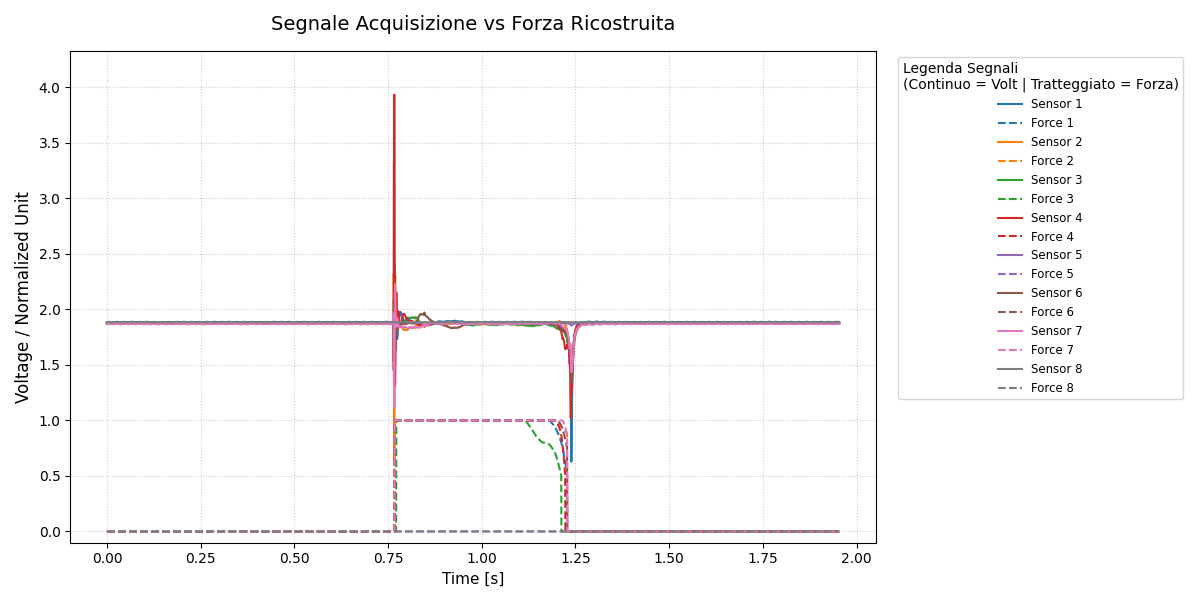
\includegraphics[width=1\textwidth]{ToccoForte.png}\\[0.3cm]
                    \caption{Prova di pressione forte sulla superficie}
                    \label{fig:PressioneForte}
                \end{figure}

                In Figura~\ref{fig:PressioneForte} viene illustrata la risposta del sistema a una pressione marcata. La marcata variazione di ampiezza nei 
                segnali di tensione (linea continua) evidenzia un picco iniziale in prossimità del valore fondo scala di $4.096\,\mathrm{V}$. Il valore di forza 
                relativa ricostruita (linea tratteggiata) segue fedelmente l'evoluzione temporale della sollecitazione: al superamento della soglia di attivazione 
                la variabile viene incrementata fino al plateau, per poi iniziare il decremento non appena il segnale rientra nelle condizioni di riposo, confermando
                il corretto funzionamento della logica di rilevamento del rilascio.

                \vspace{0.5cm}
                %Tocco Leggero
                \begin{figure}[H]
                    \centering
                    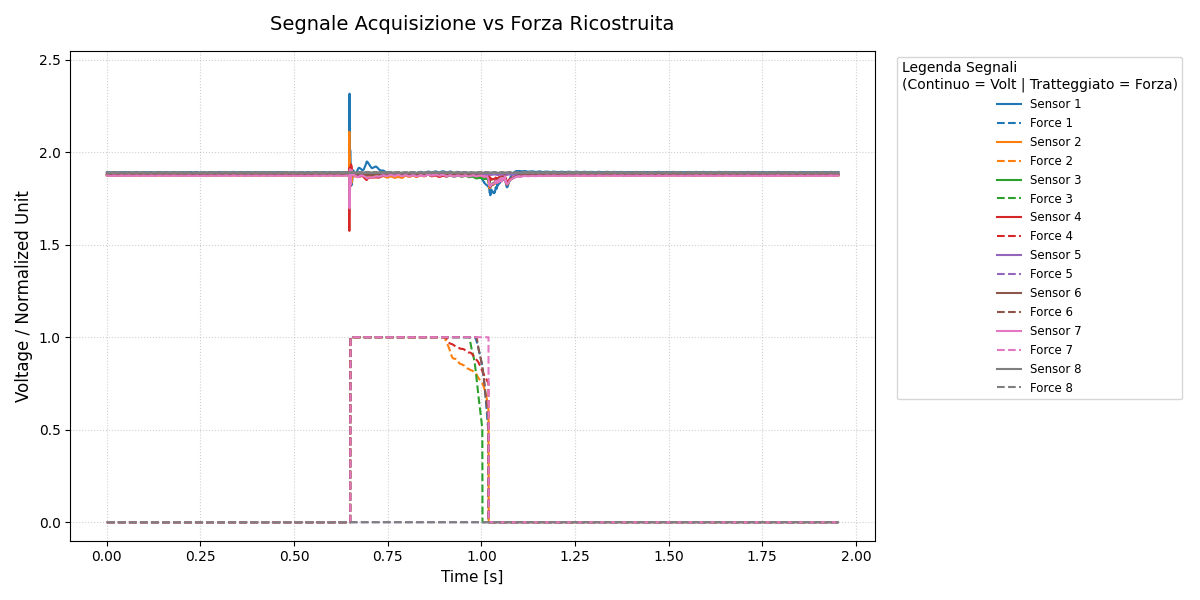
\includegraphics[width=1\textwidth]{ToccoLeggero2.png}\\[0.3cm]
                    \caption{Prova di pressione leggera sulla superficie}
                    \label{fig:PressioneLeggera}
                \end{figure}

                In Figura~\ref{fig:PressioneLeggera} viene illustrata la risposta del sistema a una sollecitazione di debole intensità (tocco leggero). 
                A differenza del caso precedente, i segnali in tensione (linea continua) mostrano un'escursione contenuta, raggiungendo un picco di 
                ampiezza ridotta attorno ai $2.3\,\mathrm{V}$, ben al di sotto del limite di saturazione dell'ADC. Ciononostante, il valore di forza 
                relativa ricostruita (linea tratteggiata) viene generato e mantenuto in modo stabile per l'intera durata del contatto, per poi azzerarsi 
                gradualmente in corrispondenza della fase di rilascio. Tale comportamento dimostra un'elevata sensibilità dell'algoritmo e la capacità 
                di discriminare con precisione anche eventi di pressione lievi rispetto al rumore di fondo.

                \vspace{0.5cm}
                %Tocco Prolungato
                \begin{figure}[H]
                    \centering
                    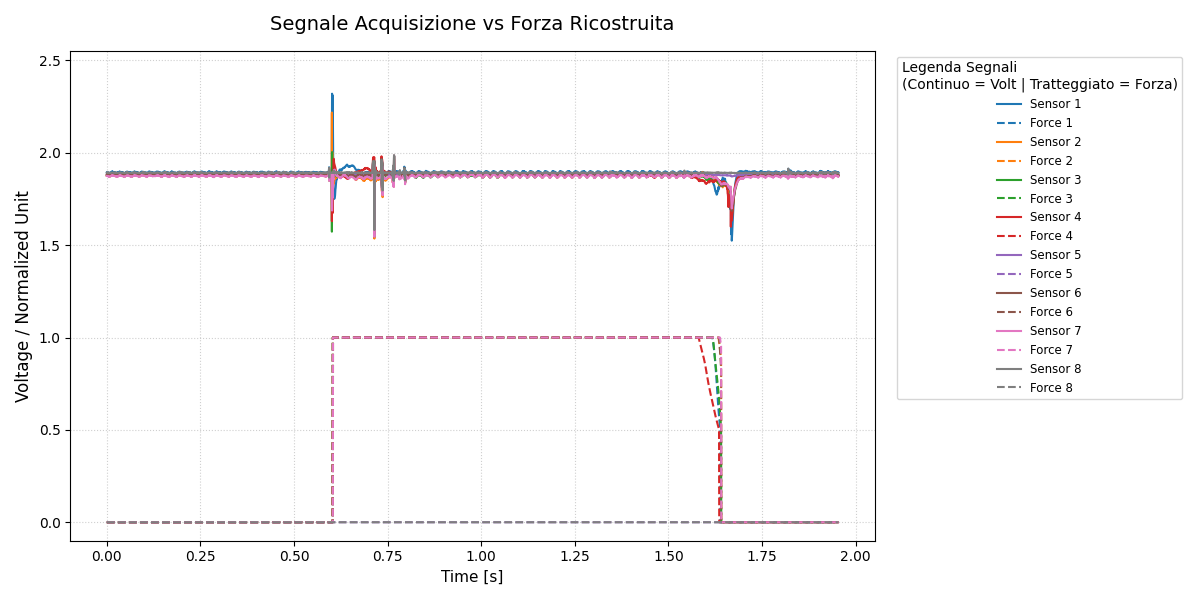
\includegraphics[width=1\textwidth]{PressioneProlungata.png}\\[0.3cm]
                    \caption{Prova di pressione prolungata sulla superficie}
                    \label{fig:PressioneProlungata}
                \end{figure}

                In Figura~\ref{fig:PressioneProlungata} viene analizzata la risposta del sistema a una sollecitazione meccanica mantenuta nel tempo 
                (pressione prolungata). Dal tracciato in tensione (linea continua) si nota come, subito dopo il transitorio d'attacco iniziale, attorno a 
                $t = 0.6\,\mathrm{s}$, si verifichi una serie di oscillazioni ad alta frequenza e di breve durata (riconducibili a un disturbo elettrico di 
                spuria o a transitori meccanici sulla matrice). Un aspetto fondamentale è rappresentato dalla robustezza del ricostruttore: l'algoritmo di 
                filtrazione ed elaborazione dello stato filtra efficacemente tali spike, evitando che il disturbo alteri la stima della forza relativa 
                (linea tratteggiata). Quest'ultima viene infatti commutata al valore massimo e mantenuta perfettamente stabile per oltre un secondo, fino al 
                netto decremento in corrispondenza del rilascio finale attorno a $t = 1.6\,\mathrm{s}$.

                \vspace{0.5cm}
                %Doppio Tocco
                \begin{figure}[H]
                    \centering
                    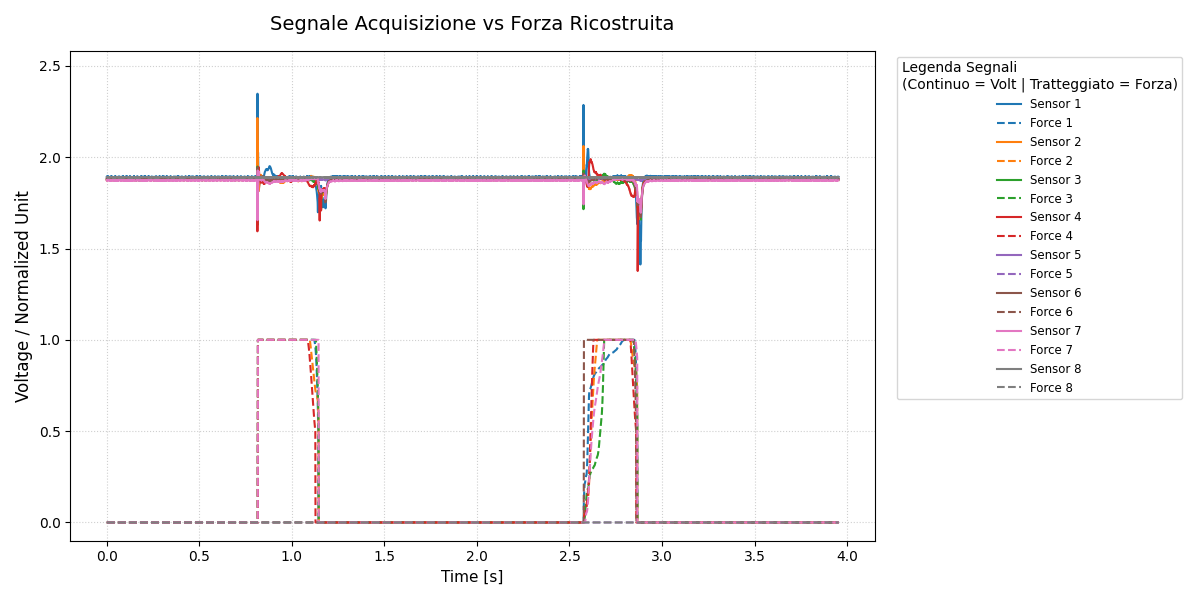
\includegraphics[width=1\textwidth]{DoppioTocco.png}\\[0.3cm]
                    \caption{Prova di pressione doppia sulla superficie}
                    \label{fig:PressioneDoppia}
                \end{figure}

                In Figura~\ref{fig:PressioneDoppia} viene illustrata la risposta del sistema a una sequenza di due sollecitazioni meccaniche distinte e ravvicinate 
                nel tempo (doppio tocco). Il primo evento si manifesta attorno a $t = 0.8\,\mathrm{s}$, dove il segnale in tensione (linea continua) genera il picco 
                d'attacco iniziale per poi attivare la ricostruzione della forza relativa (linea tratteggiata); al successivo rilascio ($t \approx 1.1\,\mathrm{s}$), 
                la variabile di forza viene riazzerata con decisione, riportando il sistema allo stato di riposo.
                La seconda sollecitazione, applicata a $t \approx 2.5\,\mathrm{s}$, evidenzia la capacità dell'algoritmo di gestire correttamente eventi consecutivi 
                senza incorrere in derive dello stato interno o falsi positivi. A differenza di quanto osservato nel caso della pressione prolungata — in cui i veloci 
                transitori ad alta frequenza non soddisfavano i criteri di rilascio, in questa prova l'intervallo temporale tra i due tocchi consente al segnale di 
                stabilizzarsi al di sotto della soglia di riposo per un numero di campioni sufficiente. Ciò permette il rispetto della condizione definita da 
                \texttt{release\_ratio} e il superamento della finestra di guardia \texttt{sample\_after\_release}. Di conseguenza, la macchina a stati finiti 
                resetta correttamente lo stato globale, consentendo il Rilevamento immediato e riproducibile del secondo impulso di pressione.
                \vspace{0.5cm}

        \subsection{Conclusioni sperimentali}       
            L'analisi svolta sulle diverse tipologie di sollecitazione meccanica ha permesso di convalidare sperimentalmente l'efficacia della catena di 
            acquisizione e dell'algoritmo di elaborazione implementato. I risultati ottenuti evidenziano in particolare tre aspetti fondamentali:

                \begin{itemize}
                    \item \textbf{Elevata dinamica e sensibilità:} Il sistema dimostra un ampio intervallo operativo, risultando in grado di gestire 
                    sollecitazioni ad elevata intensità prossime alla saturazione dell'ADC ($4.096\,\mathrm{V}$) senza incorrere in instabilità 
                    numeriche, così come tocchi di debole ampiezza ($2.3\,\mathrm{V}$), garantendo sempre una ricostruzione attendibile del profilo 
                    di forza.
                    
                    \item \textbf{Robustezza e filtraggio dei disturbi:} L'azione combinata del filtro passa-basso esponenziale e della stima 
                    dinamica dell'offset (\texttt{adaptive\_offset}) garantisce l'immunità del sistema da spike ad alta frequenza, rumore elettrico 
                    di spuria e derive della linea di base, evitando la generazione di falsi positivi o transizioni indesiderate della macchina a stati.
                    
                    \item \textbf{Gestione deterministica degli eventi:} La logica di decisione basata sui parametri \texttt{min\_press\_sensors}, 
                    \texttt{release\_ratio} e sulla finestra di guardia \texttt{sample\_after\_release} assicura un comportamento deterministico. 
                    Ciò permette sia di discriminare efficacemente transitori rapidi durante sollecitazioni prolungate, sia di riarmare prontamente 
                    lo stato del sistema per la rilevazione di impulsi multipli e ravvicinati nel tempo.
                \end{itemize}

            Nel complesso, le prove eseguite confermano che l'algoritmo soddisfa i requisiti di tempo reale e stabilità necessari per l'impiego della 
            matrice di sensori piezoelettrici in applicazioni di sensibilità tattile e robotica.
    \newpage                
    \section{Contributo personale e considerazioni conclusive}

            Il lavoro descritto in questa tesi si è concentrato sull'implementazione su microcontrollore di un algoritmo per la ricostruzione in tempo reale
            della forza relativa a partire dai segnali acquisiti da una pelle artificiale piezoelettrica. L'attività ha riguardato principalmente lo sviluppo 
            e l'integrazione della catena di elaborazione, dall'acquisizione dei segnali fino alla ricostruzione della forza e alla trasmissione dei risultati al PC.

            Gli strumenti hardware utilizzati, costituiti dal dito siliconico con pelle artificiale, dai sensori piezoelettrici e dall'interfaccia elettronica di 
            acquisizione, sono stati sviluppati presso l'Università di Genova dal gruppo di ricerca del Cosmic Lab. In questa tesi tali dispositivi sono stati 
            utilizzati come piattaforma di acquisizione, mentre il contributo personale si è concentrato sullo sviluppo software e firmware necessario alla 
            realizzazione del sistema di ricostruzione in tempo reale.

            In particolare, è stata inizialmente analizzata e verificata l'acquisizione dei segnali provenienti dagli otto sensori piezoelettrici, procedendo 
            successivamente all'implementazione e alla verifica offline dell'algoritmo di ricostruzione in ambiente Python. L'algoritmo è stato quindi portato 
            dal linguaggio Python al linguaggio C e integrato nel firmware del microcontrollore STM32H742, mantenendone la logica di elaborazione e verificando 
            la corrispondenza tra le due implementazioni.

            Il lavoro ha inoltre riguardato la gestione dell'acquisizione tramite interfaccia SPI, l'elaborazione dei dati direttamente sul microcontrollore, 
            la costruzione e la trasmissione dei pacchetti tramite UART e lo sviluppo del programma Python per la ricezione, conversione e visualizzazione dei 
            dati. È stata infine introdotta la possibilità di modificare i principali parametri del ricostruttore tramite comunicazione seriale, facilitando 
            le successive operazioni di taratura e sperimentazione.

            L'attività svolta ha permesso di approfondire tematiche relative alla programmazione in C e Python, all'interfacciamento tra microcontrollore e 
            periferiche di acquisizione, all'elaborazione digitale dei segnali e allo sviluppo di sistemi embedded per applicazioni in tempo reale. Il sistema 
            finale consente di eseguire direttamente a bordo del microcontrollore la ricostruzione della forza relativa e di rendere disponibili al PC sia i 
            dati acquisiti sia il risultato dell'elaborazione.

            Le prove sperimentali hanno infine permesso di valutare il comportamento del sistema in presenza di differenti condizioni di pressione, verificando 
            la risposta del ricostruttore e la corretta integrazione delle diverse componenti sviluppate.
    \newpage            
    \section{Riferimenti bibliografici}



\end{document}